\chapter{Methods}
\section{Thermocouple Array}
Our temperature sensor is located at Banner Creek Summit in central Idaho. This location has an elevation of about 7,040 feet above sea level and is proximal to Idaho State Highway 21. The area around Banner Summit receives an average of 1.9 meters of snow each year and frequently experiences extreme low temperatures as low as -40\textdegree C. The 2018 -- 2019 winter season experienced an above-average snowfall, with a peak snow water equivalent (SWE) measured at Banner Summit at 120\% of average. Site visits occurred on a biweekly basis unless weather or road closures forbid access. During each visit, data was collected from the instrument and snow samples were collected for stable water isotope analysis.

The structure of our sensor is comprised of a steel, rectangular frame with thin, metal cables running horizontally in 5cm increments (Fig. \ref{fig:Banner_Sensor}). A single Omega Type T thermocouple is attached to each wire, a quarter distance between the two support posts, which forms a vertical array of temperature sensors spaced 5cm apart, up to 2.5m above the ground. There were two thermocouples buried in the soil at 10cm and 5cm below ground. The buried 10cm thermocouple was installed directly adjacent to a thermistor (Campbell Scientific T107). The 53 thermocouples were multiplexed using a Campbell Scientific AM32 to a Campbell Scientific CR1000 data logger. Temperature measurements were recorded every 5 minutes. The design for this sensor came from Charlie Luce and Tom Black at the USFS and it was based off an existing sensor installed at Bogus Basin, near Boise, ID. 

A Micro-Specialties satellite telemetry system was installed during the 2020 water year so that data were accessible in near-real time. Data was transmitted every six hours using an hourly average from the measurements taken the hour before each transmit.

 \begin{figure}[H]
    \centering
    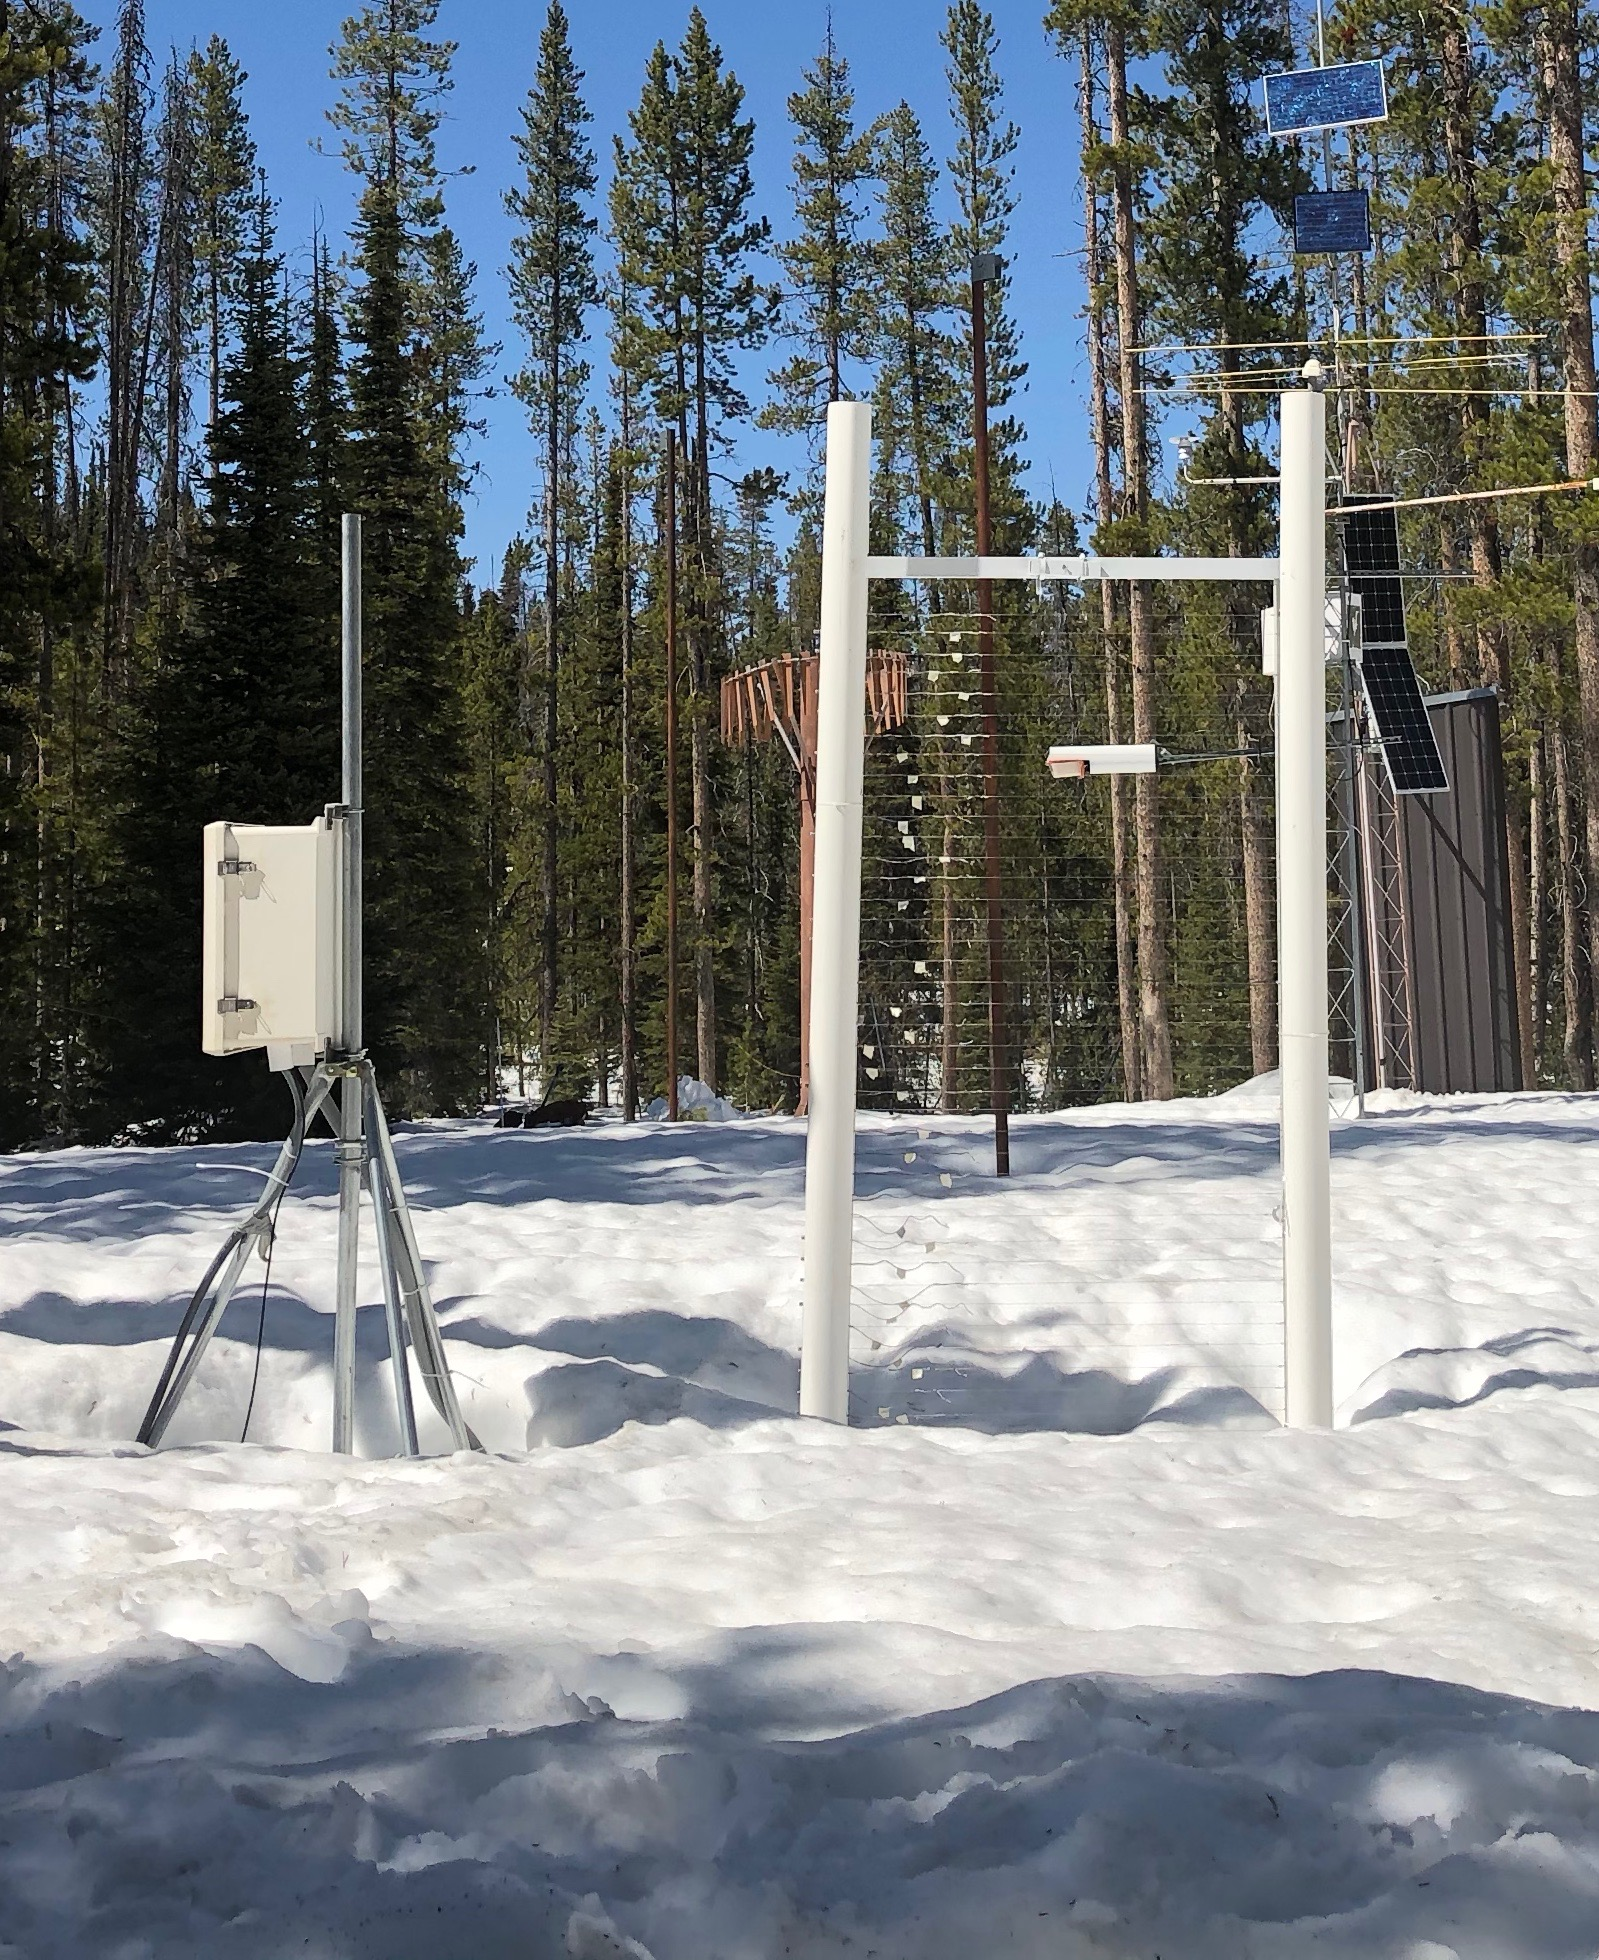
\includegraphics[width=0.7\linewidth]{figures/Banner_Sensor.jpeg}
    \caption{Picture of the instrument installed at Banner Creek Summit.}
    \label{fig:Banner_Sensor}
 \end{figure}
 
\section{Temperature Gradient Analysis}
In this analysis, we calculated the hourly average temperature gradients in the upper 25cm and the lowest 20cm of the snowpack using a first-order polynomial regression between depth and temperature (Figure \ref{fig:TempGrad_Ex}). The slope of each polynomial, i.e., the temperature gradients during 2019 in the upper 25cm and lowest 20cm, are shown in Figures \ref{fig:WY2019_GradMaster} - \ref{fig:Mar_L20_RDH}. This was done in MATLAB using the built in function called polyfit. 

There are three significant features observed from this dataset: 1) a gradient in the lower 20cm, which is the location of observed depth hoar and the depth over which avalanche forecasters are most interested in tracking the temperature gradient, 2) a near surface temperature gradient that changes diurnally, and 3) a snow surface temperature that is below the air temperature much of the time, likely due to longwave emission and sublimation. 

Data in the upper 25cm are selected because solar radiation penetrates between ~20 - 30cm depth. Additionally, the Idaho Transportation Department avalanche forecasters are primarily interested in temperature gradients in the upper 25cm, and at the base of the snowpack. The snow surface for the upper 25cm calculation is measured by the nearby SNOTEL site. Snow bridging increases the uncertainty of the temperature gradient measurements in the upper 25cm, but has a minimal impact on measurements deeper in the snowpack. The lowest 20cm are selected because there was an observed change in snow structure in this layer during December.

The temperature gradient analysis focuses on three subsets from the 2018--2019 winter season. These three subsets are selected because they illustrate critical elements of how temperature gradients evolve throughout the season. An early-season subset between November 31 to December 28 shows large temperature gradients throughout the shallow snowpack; observations made in snowpits on these two dates indicate depth hoar formation. A mid-season subset during February shows extreme cold events and record amounts of snowfall; the lowest portion of the snowpack is well insulated and does not experience critical temperature gradients. The late-season subset during March shows the snowpack as it reaches isothermal conditions.  

Temperature gradients at the top of the snowpack change diurnally because it is not completely insulated from the air. In cold, alpine environments such as Banner Summit, there was often extreme temperature gradients in the top 25cm that can lead to the formation of faceted snow. However, the diurnal nature of the upper 25cm often means that critical temperature gradients are not sustained long enough to produce faceted snow forms. The below analysis focuses on the upper 25cm because this is the extent of solar radiation penetration into the snowpack.  

\begin{figure}[H]
    \centering
    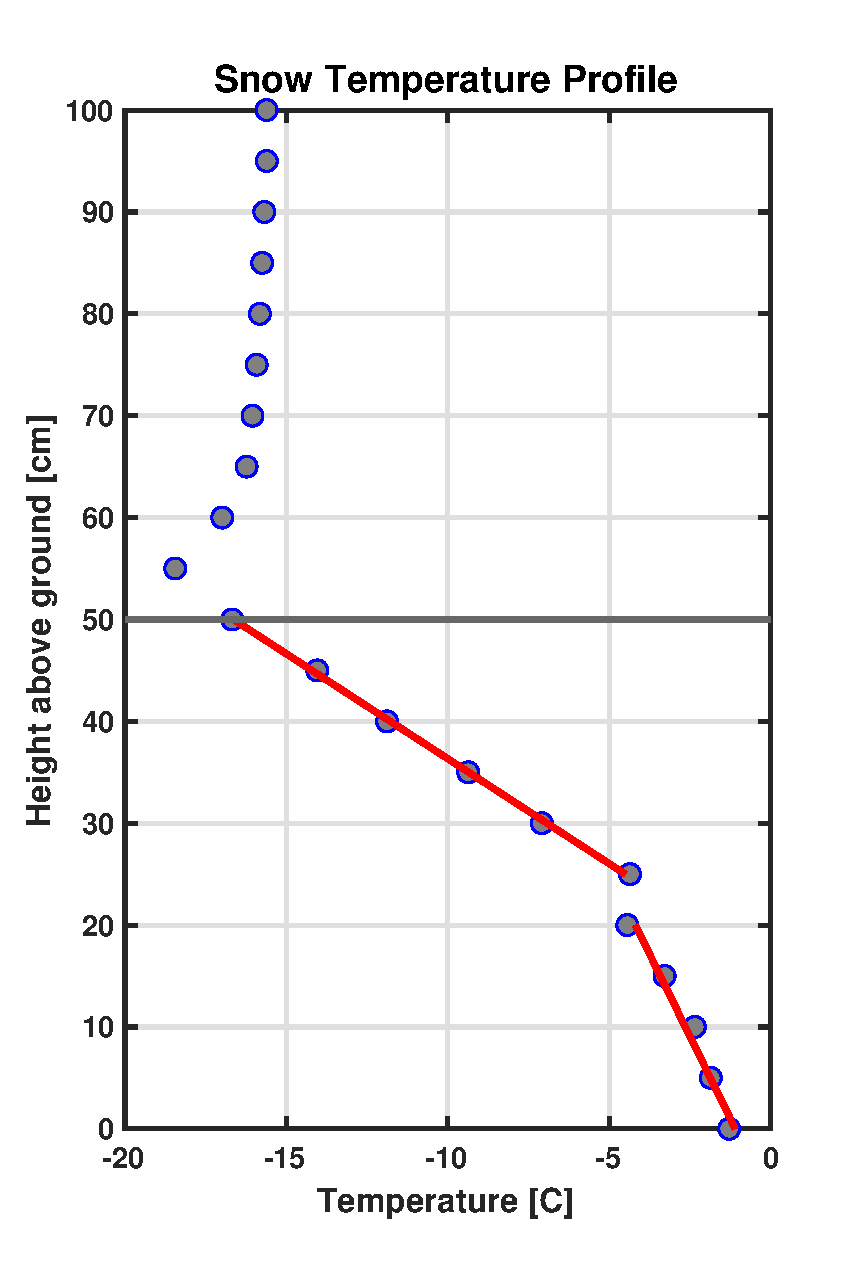
\includegraphics[width=1\linewidth]{figures/TempGrad/TempGrad_Ex.eps}
    \caption{Examples of a first order regression fit to the upper 25cm and lowest 20cm. The snow surface, as measured by the Banner Summit SNOTEL site is the horizontal, dark gray line which marks the upper limit (snow depth) of the upper 25 cm interval. The two figures are from two time periods during 2019 and illustrate differences between a shallow and a deeper snowpack. Snow accumulation on the temperature sensors is likely occurring between 120-145cm in the figure on the right.}
    \label{fig:TempGrad_Ex}
\end{figure}


 
 